\chapter{Der Residuensatz}\label{sec:Residuensatz}
Die Funktion $f(z)$ der komplexen Zahl $z=x+iy$ schreiben wir als Summe des
Real- und Imaginärteils $f(z)=u(x,y)+iv(x,y)$.
\begin{example}{Komplexe Funktionen}
  Verifiziere:
  \[ z^2=\underbrace{(x^2-y^2)}_{u(x,y)}+\underbrace{i2xy}_{v(x,y)}\]
  \[\sin(z)=\underbrace{\sin(x)\cosh(y)}_{u(x,y)}+i\cdot\underbrace{\cos(x)\sinh(y)}_{v(x,y)}\]
\end{example}

\begin{wrapfigure}[12]{l}{0.45\textwidth}
 \begin{center}
  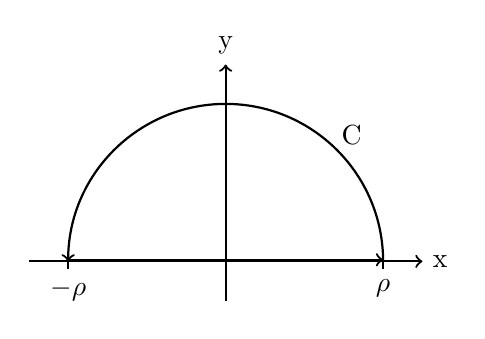
\begin{tikzpicture}[thick]
   \draw[->] (-2.5,0) -- (2.5,0) node[right] {x};
   \draw[->] (0,-.5) -- (0,2.5) node[above] {y};
   \draw[->] (-2,0.02) -- (2,0.02);
   \draw[->] (2,0) arc (0:180:2);
   %
   \draw (-2.,0) -- (-2.,-.1) node[below] {$-\rho$};
   \draw (2.,0) -- (2.,-.1) node[below] {$\rho$};
   \node at (1.6,1.6) {C};
   %
  \end{tikzpicture}
  \caption{Integrationsweg in der komplexen Ebene.\label{fig:Halbkreis}}
 \end{center}
\end{wrapfigure}
Ein Integral im Reellen, also z.B. $I=\int f(x)dx$, wird im komplexen zu einem
Linienintegral im zweidimensionalen Raum der durch $x,y$ aufgespannt wird.
Deshalb müssen wir zusätzlich noch den Integrationsweg angeben. In
Parameterform würde das bedeuten, wir müssen die Funktionen $x(s)$ und $y(s)$
angeben für ein Intervall von $s$.

Wir sind speziell an geschlossenen Intagrationswegen in der komplexen Ebene interessiert:
$I=\oint f(z)dz$, wie z.B. dem geschlossenen Halbkreis in Abbildung
\ref{fig:Halbkreis}. Auf diesem Integrationsweg wollen wir das Integral der Funktion
\[f(z)=\frac{e^{ikz}}{z^2+\Gamma^2}\]
angeben. Mit $z=\rho e^{i\varphi}$ ist $dz=e^{i\varphi}d\rho+i\rho
e^{i\varphi}d\varphi$.  Damit setzt sich das Integral aus zwei Anteilen
zusammen, das Integral über die reelle Achse von $-\rho$ bis $\rho$ und das
über den Halbkreis
\[\oint f(z)dz=\int\limits_{\substack{-\rho\\ (dy=0)}}^{\rho}\frac{e^{ikx}}{x^2+\Gamma^2}dx+
  \int\limits_{\substack{0\\(d\rho=0)}}^{\pi}\frac{e^{i\varphi}
  e^{i\rho k\cos(\varphi)-\rho k\sin(\varphi)}}{\rho^2e^{i2\varphi}+\Gamma^2}d\varphi
\]
Dabei wird als Parameter $s$ im ersten Summanden $x$ benutzt, denn auf dem
Teilstück des Wegs ist $y=0$. Im zweiten Summanden hingegen ist $\rho=const.$
und damit $\varphi$ als Parameter zu nehmen.

Im Limes $\rho\rightarrow\infty$ verschwindet der zweite Summand in obiger
Gleichung und wir erhalten
\[\lim_{\rho\rightarrow\infty}\oint f(z)dz=
  \int\limits_{\substack{-\rho\\ (dy=0)}}^{\rho}\frac{e^{ikx}}{x^2+\Gamma^2}dx=
\int\limits_{\substack{-\rho\\ (dy=0)}}^{\rho}\frac{\cos(kx)}{x^2+\Gamma^2}dx=\frac{\pi}{\Gamma}e^{-k\Gamma}
\]
Für die Berechnung von Integralen dieser Art benutzen wir den {\it
Residuensatz}. Dazu müssen wir noch den Begriff der Pole einer Funktion $f(z)$
klären. Die Funktion $f(z)$ hat an der Stelle $z=z_r$ einen {\it Pol 1. Ordnung}, wenn gilt
\[\lim_{z\rightarrow z_r}(z-z_r)f(z)\ne 0,\]
oder einen {\it Pol m-ter Ordnung}, wenn gilt
\[\lim_{z\rightarrow z_r}(z-z_r)^mf(z)\ne 0.\]
Die den Polen m-ter Ordnung zugeordneten Residuen sind definiert als
\begin{equation}
  \text{Res }\left.f(z)\right|_{z=z_r}=\lim_{z\rightarrow z_r}\frac{1}{(m-1)!}
    \frac{d^{m-1}}{dz^{m-1}}\left[(z-z_{r})^{m}f(z)\right]
  \label{eq:Residuum}
\end{equation}

Nun sind wir in der Lage den Residuensatz zu formulieren.
\begin{satz}{Residuensatz}
  Der Wert eines geschlossenen Integrals in der Ebene ist gleich dem $2\pi
  i$-fachen der Summe der umschlossenen Residuen.
  \begin{equation}
    \oint f(z)dz=2\pi i\sum\limits_{\substack{r=1\\ (z_r\text{ innerhalb }C)}}\text{Res }\left.f(z)\right|_{z=z_r} 
      \label{eq:Residuensatz}
  \end{equation}
\end{satz}

